\documentclass{article}
\usepackage[utf8]{inputenc}
\usepackage{listings}
\usepackage{xcolor}
\usepackage{subcaption}
\usepackage{minted}

\definecolor{codegreen}{rgb}{0,0.6,0}
\definecolor{codegray}{rgb}{0.5,0.5,0.5}
\definecolor{codepurple}{rgb}{0.58,0,0.82}
\definecolor{backcolour}{rgb}{0.95,0.95,0.92}
\usepackage{color}   %May be necessary if you want to color links
\usepackage{hyperref}
\usepackage{graphicx}
\hypersetup{
    colorlinks=true, %set true if you want colored links
    linktoc=all,     %set to all if you want both sections and subsections linked
    linkcolor=black,  %choose some color if you want links to stand out
    urlcolor=blue,
}
\lstdefinestyle{mystyle}{
    backgroundcolor=\color{backcolour},   
    commentstyle=\color{codegreen},
    keywordstyle=\color{magenta},
    numberstyle=\tiny\color{codegray},
    stringstyle=\color{codepurple},
    basicstyle=\ttfamily\footnotesize,
    breakatwhitespace=false,         
    breaklines=true,                 
    captionpos=b,                    
    keepspaces=true,                 
    numbers=left,                    
    numbersep=5pt,                  
    showspaces=false,                
    showstringspaces=false,
    showtabs=false,                  
    tabsize=2
}

\lstset{style=mystyle}


\title{SMBUD}
\author{Filippo Lazzati, Martina Magliani, Christian Grasso, Sofia Martellozzo, Giacomo Lombardo}
%\date{October 2021}

\begin{document}
\thispagestyle{empty}
\begin{titlepage}
    \begin{center}
       %\vspace*{2cm}
       {\Huge \textbf{SMBUD}} %%Replace this with the Title of your research
       \vspace{0.5cm}
       \\
    \begin{LARGE}
        {Vaccination and Certificates}
        \vspace{1.0cm}
        \\
        {\textit{Specification, Entity-Relationship model and MongoDB CRUD operations}}
           
\includegraphics[width=13cm]{logo/polimi.png}
          \vspace{1.5cm}\\
                  Filippo Lazzati (10629918) - Martina Magliani (10682333) - Christian Grasso (10652464) - Sofia Martellozzo (10623060) - Giacomo Lombardo (10674987)\\
       {Year: 2021/2022}
    \end{LARGE}  
   \end{center}
\end{titlepage}
\newpage
\tableofcontents %this command creates an index
\newpage
\section{Problem specification}
The purpose of this project is to build an information system that is able to manage pandemic information for a given country. In particular, such system must be scalable enough to manage all the information about COVID-19 tests and vaccinations, and it should provide data at the granularity level required by a business perspective. Moreover, the storage system should be flexible enough in order to comply with the expiration dates of the certificates and, potentially, with the evolution of the rules.\\
Since \verb|MongoDB| is a document-oriented database with the property of being schema-less, it perfectly matches this use case. Furthermore, because of its document-oriented structure, it solves the impedance-mismatch problem and, thus, allows to retrieve data also through object-oriented code. The main drawback is the duplication of the data, which is, in a measure, acceptable in the scenario of the certificates.
\section{Hypotheses} \label{hypotheses}
The database is implemented under the following hypotheses:
\begin{itemize}
    \item for each person owning a certificate some demographic details are known;
    \item for each person owning a certificate is also known an emergency contact;
    \item there are 3 different ways through which a person can receive a certificate:
    \begin{enumerate}
        \item healing from the disease; the validity of the certificate is fixed and assumed to be of 6 months after the recovery. A recovery is certified through one negative test after a positive one;
        \item taking at least 1 dose of vaccine; see below for details about the validity of the certificate;
        \item taking a test; the validity varies between the 48 and the 72 hours;
    \end{enumerate}
    \item by definition, a certificate is valid if it contains at least one valid vaccine/test or a certified recovery from the illness;
    \item each person can receive 0, 1, 2 or 3 doses of vaccine (it should be noticed that, up to now, the fourth dose is not considered; however, since \verb|MongoDB| is schema-less, the introduction of the n-th dose can be easily introduced in the database);
\item there are various types of vaccine, each one with different characteristics in terms of the validity of the certificate (here, for the sake of simplicity, the vaccines are listed using the name of the brand):
\begin{enumerate}
    \item Pfizer/BioNTech, which provides a valid certificate after 15 days from the first dose and up to 9 months after the administration of the second dose;
    \item Moderna, whose certificates have the same characteristics of the Pfizer's one;
    \item AstraZeneca, whose certificates have the same characteristics of the Pfizer's one;
    \item Johnson \& Johnson, which provides a valid certificate after 15 days from the first dose and valid for 6 months (for the time being we assume that no person can take more than one vaccine dose if she has taken the Johnson \& Johnson vaccine as the first one);
   \item Sputnik, which does not provide any valid certificate because of UE regulations.
\end{enumerate}
It should be noticed that the flexibility offered by a schema-less database like \verb|MongoDB| can be very useful in this case, since the details of the certificates with regards to the type of vaccine can change over time;
\item the validity of the first dose of vaccine expires 3 months in case the person does not undergo a second dose;
\item each vaccine dose is characterized by:
\begin{enumerate}
    \item the name of the brand that produces it;
    \item the name of the vaccine;
    \item the lot of the vaccine;
    \item the production date;
\end{enumerate}
\item a temporary certificate can be obtained also via a COVID-19 test, which can be:
\begin{enumerate}
    \item rapid, which provides a valid certificate for 48 hours;
    \item PCR, which provides a valid certificate for 72 hours;
    \end{enumerate}
\item each test is registered when the result is available and is characterized by the type of the test (rapid/PCR);
\item vaccines and COVID-19 tests can be done in various locations. Each location is characterized by:
\begin{enumerate}
    \item the name of the hospital/health service (or whatever other place like, for instance, a supermarket or the hairdresser) where the vaccine (test) has been administered (taken);
    \item the type of the service (e.g. hospital, local healthcare facility, pharmacy, supermarket etc.);
    \item a full text description of such place;
    \item the address of the location;
    \item the GPS coordinates of the location;
    \item optionally, the department (this can be present only for hospitals and big health structures);
\end{enumerate}
\item vaccines and tests are administered by authorized health personnel such as doctor and nurses, characterized by name, surname, fiscal code and the position (e.g. nurse, doctor);
\item for each vaccine/test that is administered, the certificate includes the health personnel attending the administration;
\item a doctor/nurse can administer a vaccine in a different place than the workplace (e.g. supermarket or another health structure);
\item each certificate has a unique code of 6 digits that allows to retrieve it; such code does the same job of the QR code of the \verb|GREEN| \verb|PASS|;
\item no person takes another test before that the 48h (or 72h in case of a pcr test) of a test resulted negative expire (this assumption is rather strong, but we consider it meaningful and useful, therefore we decided to add it).
\end{itemize}
\newpage
\section{Conceptual model}
The following is the Entity-Relationship (E-R) model of our database:\\ \\ \\
\vspace{1cm}
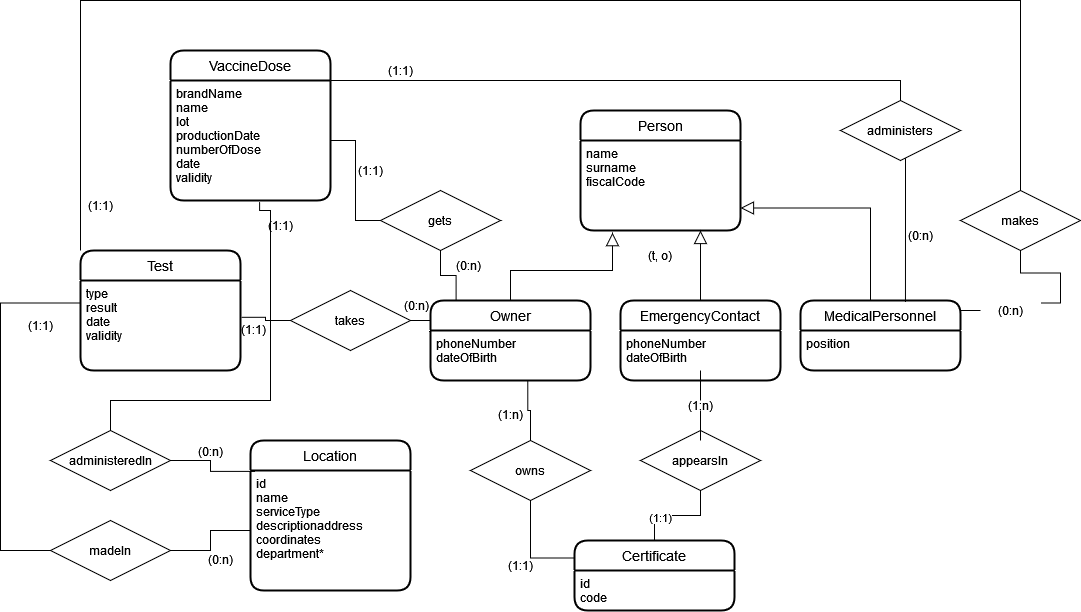
\includegraphics[trim=1cm 1cm 1cm 1cm, width=15cm]{images/e-r.png}
Notice that the optional attributes have been marked with a star (*).\\
The Entity-Relationship model contains 5 main entities, that are related to each other through various relationships.
\begin{itemize}
    \item \textit{PERSON} represents a person. Every \textit{PERSON} has a name, a surname and a fiscal code. Then there are 3 entities that inherit from \textit{PERSON}, namely \textit{OWNER}, \textit{EMERGENCYCONTACT} and \textit{MEDICALPERSONNEL}. It has been assumed that it is not relevant to insert the date of birth of the \textit{MEDICALPERSONNEL} in the certificate, and that it should be better to avoid to insert its phone number in it. Of course the attributes of \textit{PERSON} could be enlarged, but as a sample dataset we have believed that these three are enough;
    \item \textit{CERTIFICATE} represents the main concept of the whole database. The \textit{CERTIFICATE} will be the document on which we put more or less all the data we have, because the \textit{CERTIFICATE} is at the level of granularity  with which users want to work with this data. We have preferred to represent such entity with only an identifier and the unique code of 6 digits, since it acquires all the data it owns through its relationships;
    \item \textit{LOCATION} represents a place where a vaccine or a test can be done. It should be remarked that we have decided to write in detail such entity, because it is relevant for this scenario. Because of the many attributes it has, you will notice that this is the only document that has not been added to the \textit{CERTIFICATE} document to avoid a useless waste of storage space (as a matter of fact, we have assumed that the \textit{LOCATION} is relevant but it is not required so much from the "business", therefore when it is asked they can wait some additional time). The \textit{LOCATION}s will lie in a different collection;
    \item \textit{VACCINEDOSE} represents one single dose of vaccine received by a person; it has a name, the name of the brand, the lot number and the date of production;
    \item \textit{TEST} represents one single test taken by a person; it is characterised by a type (rapid or PCR), a result, a date and the validity (48 hourse or 72 hours).
\end{itemize}
Among these entities, some relations hold. In particular:
\begin{itemize}
    \item \textit{ADIMINISTERS} and \textit{MAKES} represent the relation between a medical personnel and the vaccine/test he does;
    \item \textit{GETS} and \textit{TAKES} bind a person (\textit{OWNER}) with its doses of vaccine/tests;
    \item \textit{ADMINISTEREDIN} and \textit{MADEIN} specify in which location a certain vaccine dose/test has been administered;
    \item \textit{OWNS} simply relates a person (\textit{OWNER}) to her certificate. \textbf{Notice that there is a 1-to-1 relationship between \textit{PERSON} and \textit{CERTIFICATE}: in our database, every time a person takes a test (or a vaccine dose), it is added to the same certificate of the person. In this way, there is not an annoying change of the 6-digits code (QR code) every time the certificate changes (like in GREEN PASS). If a certificate is not valid, it will be simply parsed as non-valid.}
    \item \textit{APPEARSIN} relates the \textit{EMERGENCYCONTACT}s to the certificates in which they appear as such.
\end{itemize}
\newpage
\section{Sample dataset}
\subsection{Example of documents}
The sample dataset we provide, created through some \verb|PHP| scripts, is made of the following two documents (and all the nested subdocuments). As previously said, the decision to avoid to embed the \verb|LOCATION| documents inside the \verb|CERTIFICATE| ones has been taken in order to prevent a huge and useless waste of storage space. The following is an example of a \verb|CERTIFICATE| document:
\begin{minted}{json}
{
        "code": "3U4162",
        "owner": {
            "name": "John",
            "surname": "Morris",
            "dateOfBirth": "1986-07-14",
            "fiscalCode": "JHNMRS86L14S677A",
            "phoneNumber": 3313567314
        },
        "recovered": null,
        "emergencyContact": {
            "name": "Michelle",
            "surname": "Hampton",
            "dateOfBirth": "2006-03-31",
            "fiscalCode": "MCHHPT06C71Q216S",
            "phoneNumber": 3002475590
        },
        "vaccines": [
            {
                "type": {
                    "name": "Comirnaty",
                    "brandName": "Pfizer\/BioNTech",
                    "lot": "NRZZZHOH",
                    "productionDate": "2021-03-03"
                },
                "numberOfDose": 1,
                "validity": 6480,
                "date": "2021-04-06",
                "medicalPersonnel": {
                    "name": "Peter",
                    "surname": "Davis",
                    "fiscalCode": "PTRDVS48P04L453S",
                    "position": "doctor"
                },
                "locationId": "location_949"
            },
            {
                "type": {
                    "name": "Comirnaty",
                    "brandName": "Pfizer\/BioNTech",
                    "lot": "KDTULQPG",
                    "productionDate": "2021-04-15"
                },
                "numberOfDose": 2,
                "validity": 6480,
                "date": "2021-05-01",
                "medicalPersonnel": {
                    "name": "Robert",
                    "surname": "Savage",
                    "fiscalCode": "RBRSVG76R210827S",
                    "position": "doctor"
                },
                "locationId": "location_1922"
            }
        ],
        "tests": [
            {
                "type": "pcr",
                "validity": 72,
                "result": false,
                "date": "2021-02-02",
                "medicalPersonnel": {
                    "name": "James",
                    "surname": "Williams",
                    "fiscalCode": "JMSWLM94C24X515S",
                    "position": "doctor"
                },
                "locationId": "location_1924"
            }
        ]
    }
\end{minted}
A \verb|CERTIFICATE| document is recognized (like every document in \verb|MongoDB|) by an "\_id" and contains:
\begin{itemize}
    \item a unique 6-digits code different from the "\_id", that can be used to identify the certificate (such code has the same role of the QR code in the \verb|GREEN| \verb|PASS|);
    \item the owner of the document;
    \item the emergency contact of the owner of the document;
    \item a list of all the doses of vaccine received (in this way if the rules evolve, additional doses can be added to new documents);
    \item a list of all the tests taken by the owner of the certificate.
\end{itemize}
Notice that the validity is expressed in hours; so, for instance, the Pfizer/BioNTech vaccine which gives a validity of 9 months as second dose is represented with the field: $validity = 9 * 30 * 24 = 6480$.
This is a design choice.\\ \\
\vspace{0.3cm}
On the other side, an example of \verb|LOCATION| document is the following:
\begin{minted}{json}
{
        "_id": "location_0",
        "name": "Location 0",
        "address": "VIA PANORAMICA 42, BORGO TOSSIGNANO",
        "typeOfService": "vaccinationCenter",
        "coordinates": [
            43.2881,
            12.12
        ],
        "department": null
    }
\end{minted}
It is recognized by an "\_id" and contains all the attributes identified in the conceptual model (E-R) of the data. The \verb|CERTIFICATE| documents contain links to it (when needed).
\subsection{Import the dataset}\label{import}
The sample dataset is given through two different \verb|JSON| files, "certificates.json" and "locations.json". The former contains an array of certificate documents while the latter an array of location documents. For the sake of simplicity we have decided to generate on our own the "\_id" attribute of the locations.\\
To import the dataset, you have to follow these steps (since certificates and locations are different kinds of document, they will be imported into different collections):
\begin{enumerate}
    \item open a command prompt and type \begin{lstlisting}[language=bash]
    mongod
\end{lstlisting}
\item open \verb|MongoDBCompass| and type the string "mongodb://127.0.0.1:27017/";
\item create a new database called "db" and two new collections called "certificates" and "locations" inside it;
\item import the two \verb|JSON| files "certificates.json" and "locations.json" respectively in the collections certificates and locations (exploit the \textit{ADD DATA} button).
\end{enumerate}
\section{Queries and Commands}
The following queries and commands have been developed in order to provide an example of usage of the system for typical scenarios.
\subsection{Queries}
We have identified the following queries:
\begin{enumerate}
\item \textbf{find all the people who have recovered from the disease}.\\
We simply have to check whether the "recovered" attribute is null or not:
\begin{lstlisting}
db.certificates.find({"recovered":{$ne:null}}, {"owner": 1});
    \end{lstlisting}
    \item \textbf{find all the people who have undergone 3 vaccine doses}.\\
    Thanks to the \verb|$size| operator, we can make a query on the length of an array:
    \begin{lstlisting}
db.certificates.find({vaccines: {$size: 3}}, {"owner": 1});
    \end{lstlisting}
    \item \textbf{find all the valid certificates}.\\
    According to the hypotheses (see section \ref{hypotheses}), a certificate is valid in 3 cases:
    \begin{enumerate}
            \item the owner healed from the disease (verified through a negative test after a positive one) -$>$ 6 months $\approx$ 4320 hours of validity;
        \item the owner took a (negative) test in the last hours -$>$ 48h or 72h of validity;
        \item the owner underwent at least one vaccination dose -$>$ 3 months of validity for the first dose, then the validity varies according to the type of vaccine.
    \end{enumerate}
    Therefore, we can write 3 different queries to retrieve certificates that are valid for different reasons.\\
    \begin{enumerate}
        \item Certificates of people who have recovered in the last 6 months:
    \begin{lstlisting}
db.certificates.find({"recovered": {$gte: new Date(ISODate().getTime() - 1000 * 60 * 60 * 24 * 30 * 6)}});
    \end{lstlisting}
    \item certificates of people who have taken a (negative) test in the last hours (48 or 72 according to the type of test):
    \begin{lstlisting}
db.certificates.find({$or: [
{tests: {$elemMatch: {validity: 48, result: false, date: {$gte: new Date(ISODate().getTime() - 1000 * 60 * 60 * 24 * 2)}}}}, 
{tests: {$elemMatch: {validity: 72, result: false, date: {$gte: new Date(ISODate().getTime() - 1000 * 60 * 60 * 24 * 3)}}}}]});
    \end{lstlisting}
    \textbf{N.B.:} it should be remarked that this query is correct only thanks to the assumption that states that no person can take another test while having taken a negative test in the last 48/72 hours.
    \item certificates of people who have undergone vaccination not too much time ago and therefore the certificates are valid (notice that, since the first dose gives a valid certificate after 15 days, we have to add such value in the conditions):
    \begin{lstlisting}
db.certificates.find({$or: [
    {vaccines: {$elemMatch: {validity: 2160, date: {$gte: new Date(ISODate().getTime() - 1000 * 60 * 60 * 2160 + 1000 * 60 * 60 * 24 * 15)}}}},
    {vaccines: {$elemMatch: {validity: 4320, date: {$gte: new Date(ISODate().getTime() - 1000 * 60 * 60 * 4320)}}}},
    {vaccines: {$elemMatch: {validity: 6480, date: {$gte: new Date(ISODate().getTime() - 1000 * 60 * 60 * 6480)}}}}
]});
    \end{lstlisting}
    It should be noticed that this query is not exactly correct, because there is the possibility that a person is tested positive after having received the vaccine, and thus her certificate is not valid anymore. However, for the sake of simplicity, we will check this fact with \verb|JavaScript| in the user interface.
    \end{enumerate}
    \item \textbf{find the type of vaccine which has been administered the most}.\\
    It is clear that we have to use aggregations for this query. The pipeline starts with \verb|$unwind|, which allows to expand the content of the array "vaccines"; next, \verb|$group| allows to group the documents by brandName, and finally we sort the results through \verb|$sort| and take the maximum using \verb|$limit|. 
    \begin{lstlisting}
db.certificates.aggregate([
    {
        '$unwind': {
            'path': '$vaccines'
        }
    }, {
        '$group': {
            '_id': '$vaccines.type.brandName', 
            'count': {
                '$sum': 1
            }
        }
    }, {
        '$sort': {
            'count': -1
        }
    }, {
        '$limit': 1
    }
]);
    \end{lstlisting}
    \item \textbf{find the medical personnel who has administered more vaccines}.\\This query is rather similar to the previous one; indeed, we need again to use aggregation and the pipeline proceeds along the same operators:
    \begin{lstlisting}
db.certificates.aggregate([
    {
        '$unwind': {
            'path': '$vaccines'
        }
    }, {
        '$group': {
            '_id': {
                'fiscalCode': '$vaccines.medicalPersonnel.fiscalCode', 
                'name': '$vaccines.medicalPersonnel.name', 
                'surname': '$vaccines.medicalPersonnel.surname', 
                'position': '$vaccines.medicalPersonnel.position'
            }, 
            'count': {
                '$sum': 1
            }
        }
    }, {
        '$sort': {
            'count': -1
        }
    }, {
        '$limit': 1
    }
]);
\end{lstlisting}
    \item \textbf{find the people who have taken only tests}.\\
    This query allows to retrieve all the people who have never undergone vaccination but who have taken at least one test. Since the owner of a certificate is inside the certificate, we simply have to project the owner: 
    \begin{lstlisting}
    db.certificates.find({
            "$and":[{"$expr":{$eq:[{$size:"$vaccines"},0]}},{"$expr":{$gte:[{$size:"$tests"},1]}}]
    });
\end{lstlisting}
    \item \textbf{find the 10 locations with the highest number of vaccines administered}.\\
    Like two previous queries, again we are looking for the maximum, therefore the pipeline is the same. The only difference is that now we are looking for the top 10 locations, thus the \verb|$limit| operator has a 10 instead of a 1:
    \begin{lstlisting}
    db.certificates.aggregate([
    {
        '$unwind': {
            'path': '$vaccines'
        }
    }, {
        '$group': {
            '_id': '$vaccines.locationId', 
            'count': {
                '$sum': 1
            }
        }
    }, {
        '$sort': {
            'count': -1
        }
    }, {
        '$limit': 10
    }
]);
    \end{lstlisting}
    Then the details about the locations can be retrieved by querying the \verb|locations| collection with the returned \_\verb|id|s.
    \item \textbf{find how many vaccinated people there are in the system}.\\
    For this query we use the aggregation construct; we match all the certificates with at least one vaccine dose (size greater than or equal to 1) and then we count how many certificates we have. Clearly, we have to use the \verb|certificates| collection:
\begin{lstlisting}
db.certificates.aggregate([
            {
                '$match': {
                    '$expr': {
                        '$gte': [
                            {
                                '$size': '$vaccines'
                            }, 1
                        ]
                    }
                }
            }, {
                '$count': 'numOfVaccinatedPeople'
            }
        ]);
\end{lstlisting}
    \item \textbf{find all the vaccinated people and, for each of them, the number of doses done}.\\
    We use an aggregation construct in which we apply the \verb|$project| operator to take only the persons along with the number of doses done, then we get rid of the people with 0 vaccine doses:
    \\
    \begin{lstlisting}
        db.certificates.aggregate([
            {
               '$project': {
              'person': '$owner',
                  'numberOfDoses': {
                      $size: '$vaccines'
                }
             }
         },
         {
         '$match': {
                    '$expr': {
                        '$gte': [
                                '$numberOfDoses', 1
                        ]
                    }
                }}]); 
    \end{lstlisting}
    \end{enumerate}
\subsection{Commands}
We have identified the following commands to show how the system works:\\
\begin{enumerate}
    \item \textbf{Update a certificate because of a new vaccine dose}.\\
    We use the \verb|updateOne()| function in which we look for the certificate to update through the unique 6-digits code ($\approx$ QR code) and then we push inside the \verb|vaccines| array the new dose. It should be noticed that the use of the construct \verb|$date| is essential in order to insert dates instead of strings:
    \begin{lstlisting}
        db.certificates.updateOne(
            {
                code: 'L7R43T'
                }, {
                    $push: {
                        'vaccines': {
                        'type' : {
                            'name': 'Vaxzevria',
                            'brandName': 'AstraZeneca',
                            'lot': 'K6OGB2VP',
                               'productionDate': {
                        '$date': '2021-01-07T22:13:06+01:00'
                    }
                            },
                        'numberOfDose': 1,
                        'validity': 2160,
                        'date': {
                        '$date': '2021-01-07T22:13:06+01:00'
                    },
                        'medicalPersonnel': {
                            'name': 'Harry',
                            'surname': 'Cooper',
                            'fiscalCode': 'HRRCPR45H08A966A',
                            'position': 'other'
                               },
                        'locationId': 'location_1175'
                        }
                    }
            });
    \end{lstlisting}
    \item \textbf{Update a certificate because of a new test}.\\
    This query is quite similar to the previous one: we find a certificate through the unique 6-digits code and we push into the \verb|tests| array the new test. For the sake of simplicity, the task of checking whether the owner has previous tests and whether the last test taken is positive is performed by the application; in such a case, if the new test is negative the application will automatically update the field \verb|recovered| of the document with the date of the new test.\\
    \begin{lstlisting}
        db.certificates.updateOne({
            code: 'L7R43T'
            }, {
            $push : {
                'tests': {
                    'type': 'rapid',
                            'validity': 48,
                            'result': false,
                            'date': {
                            '$date': '2021-01-07T22:13:06+01:00'},
                            'medicalPersonnel': {
                               'name': 'Albert',
                                'surname': 'Saults',
                                'fiscalCode': 'LBRSTS17S13W706O',
                                'position': 'nurse'
                                },
                            'locationId': 'location_1988'
                }
            }
        
        });
    \end{lstlisting}
    \item \textbf{insert a certificate because a new person has received the first vaccine dose or has made the first test}.\\
    In this case, the person does not have a certificate yet, therefore we exploit the \verb|insert()| function to insert a new certificate in the database (in the example Michael Penn has just taken his first vaccine dose):
    \begin{lstlisting}
db.certificates.insert({
    'code': 'QSA4GP',
    'owner': {
        'name': 'Michael',
        'surname': 'Penn',
        'dateOfBirth': '1986-06-03',
        'fiscalCode': 'MCHPNN86H03C751C',
        'phoneNumber': {
            '$numberLong': '3121784343'
        }
    },
    'recovered': null,
    'emergencyContact': {
        'name': 'Esther',
        'surname': 'Bernard',
        'dateOfBirth': '1968-06-30',
        'fiscalCode': 'STHBNR68H70R928L',
        'phoneNumber': {
            '$numberLong': '3585672957'
        }
    },
    'vaccines': [{
        'type': {
            'name': 'Janssen',
            'brandName': 'J&J',
            'lot': '5S3QLBDA',
            'productionDate': {
                            '$date': '2021-01-07T22:13:06+01:00'},
        },
        'numberOfDose': 1,
        'validity': 4320,
        'date': {
                '$date': '2021-01-07T22:13:06+01:00'},
        'medicalPersonnel': {
            'name': 'Vincent',
            'surname': 'Vang',
            'fiscalCode': 'VNCVNG55R160373I',
            'position': 'nurse'
        },
        'locationId': 'location_1006'
    }],
    'tests': []
 });
    \end{lstlisting}
\end{enumerate}
\section{User Interface}
    We have provided a demo of a User Interface in order to implement some real-life use cases and to show some meaningful interaction between the database and external applications. The demo consists of a simple client-server application implemented in \verb|node.js|, using \verb|express.js| and the \textit{MongoDB Node Driver} for the back-end and the \verb|React| framework for the front-end.\\
    The UI aims to simulate a real-life system for the verification of COVID-19 certificates: by inserting the 6-digits certification code into the system, the user will be able to verify whether the corresponding certificate is valid or not and to visualize the certificate's data. Furthermore, the UI provides some other functionalities to interact in various ways with the database, that are:
    \begin{itemize}
    \item verify whether a certificate is valid or not;
    \item insert a new vaccine or a new test in a given certificate;
    \item visualize a list of locations, their information and statistics.
    \end{itemize}
\section{User guide}
In order to run the application, you need a MongoDB database with the provided data (see Section \ref{import}) and \textit{Node.js} installed on the machine.\\
After having installed \textit{Node.js}, follow these steps to run the application:
\begin{enumerate}
    \item move to the \verb|webapp| folder;
    \item in the \verb|server| folder, edit \verb|config.env| inserting username, password and name of the database in the corresponding placeholders (remember to remove \verb|'<'| and \verb|'>'|);
    \item open the terminal in the \verb|webapp| folder;
    \item to install dependencies and build the application, run \verb|npm run build|. This command will install the necessary \textit{node modules} and will build the front-end application;
    \item to start the application, run \verb|npm start|;
    \item to use the application, open your browser and go to \verb|http://localhost:5000|.
\end{enumerate}
\textbf{N.B.:} if you are using macOS, you could be required to disable \textit{Airplay Receiver} before running the code. 
\section{References and sources}
\begin{itemize}
    \item \href{https://www.mongodb.com}{MongoDB}
    \item \href{https://app.diagrams.net}{draw.io}
    \item \href{https://nodejs.org}{node.js}
    \item \href{https://expressjs.com}{express.js}
    \item \href{https://reactjs.org/}{React}
\end{itemize}
\section{Image gallery}
In this section we include some screenshots showing the appearance of the User Interface (UI).\\Read the captions for details about what each image represents.
    \begin{figure}[ht!]
    \centering
    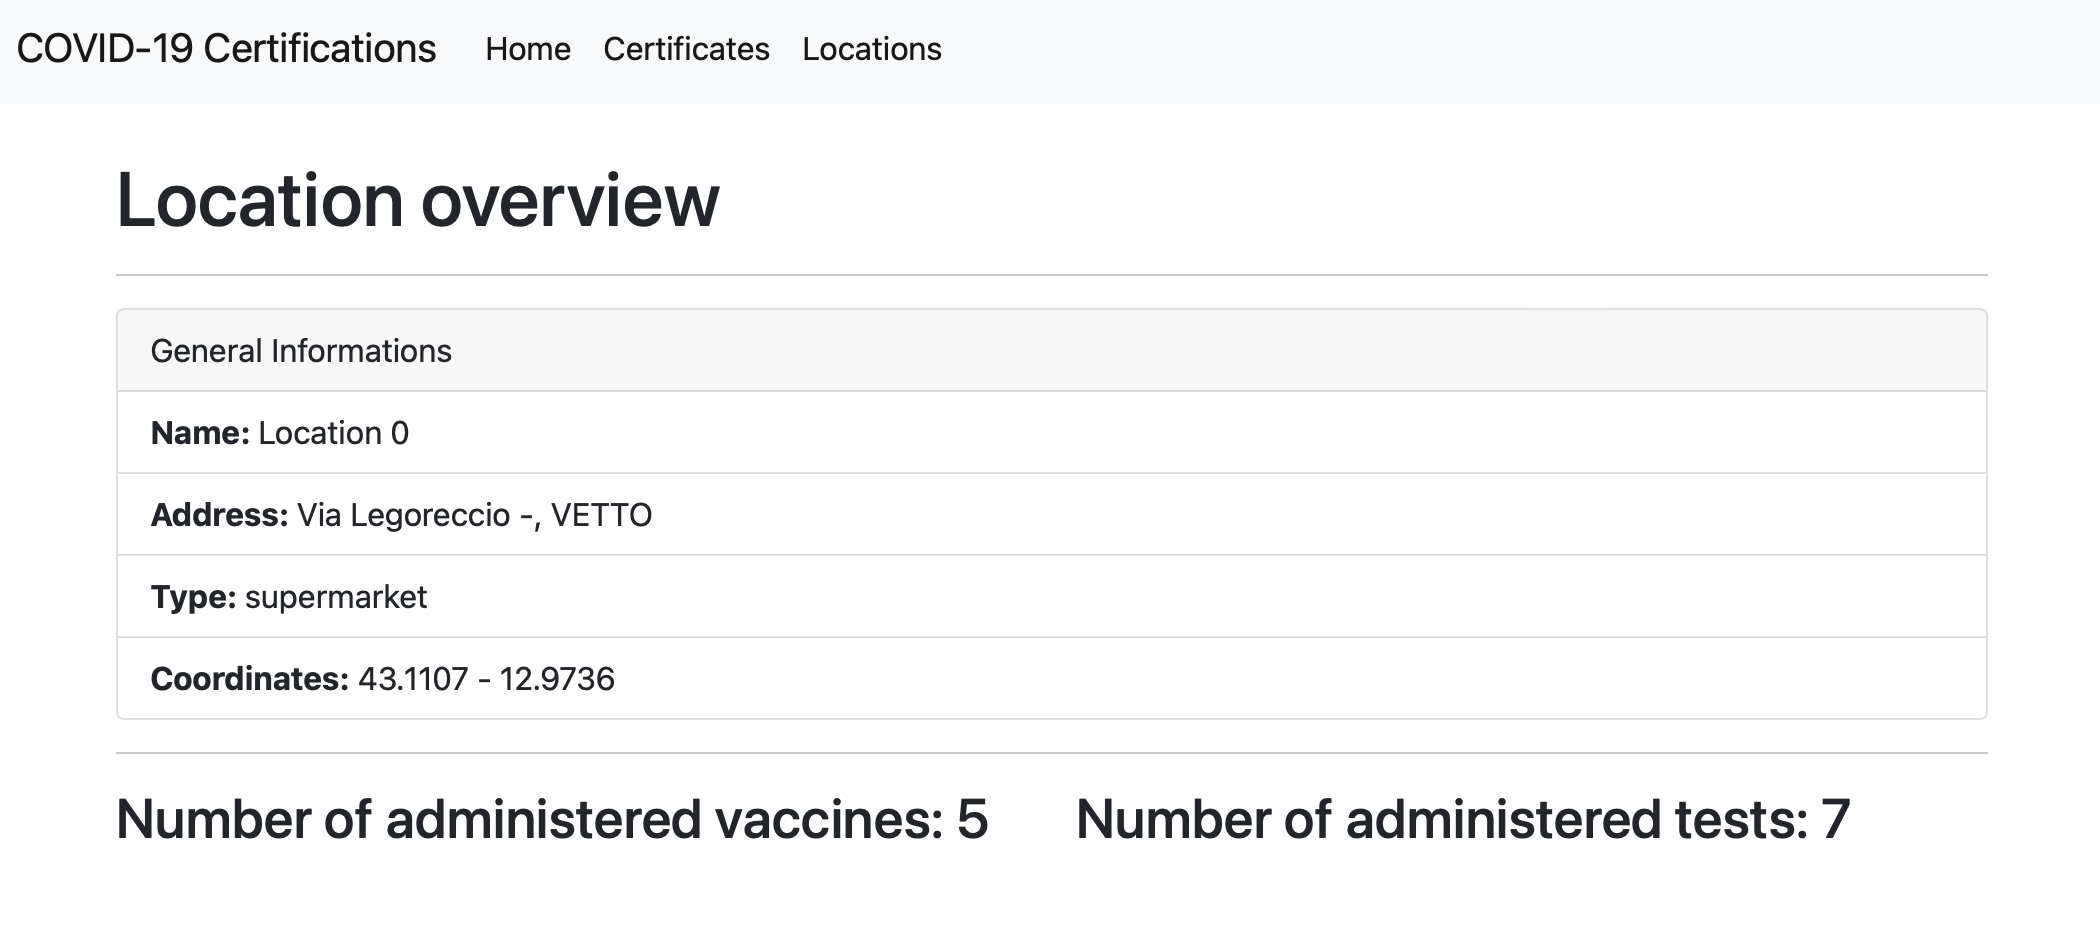
\includegraphics[scale=0.3]{screenshots/location.png}
    \caption{User interface for visualizing a location in the database.}
\end{figure}
\begin{figure}[ht!]
    \centering
    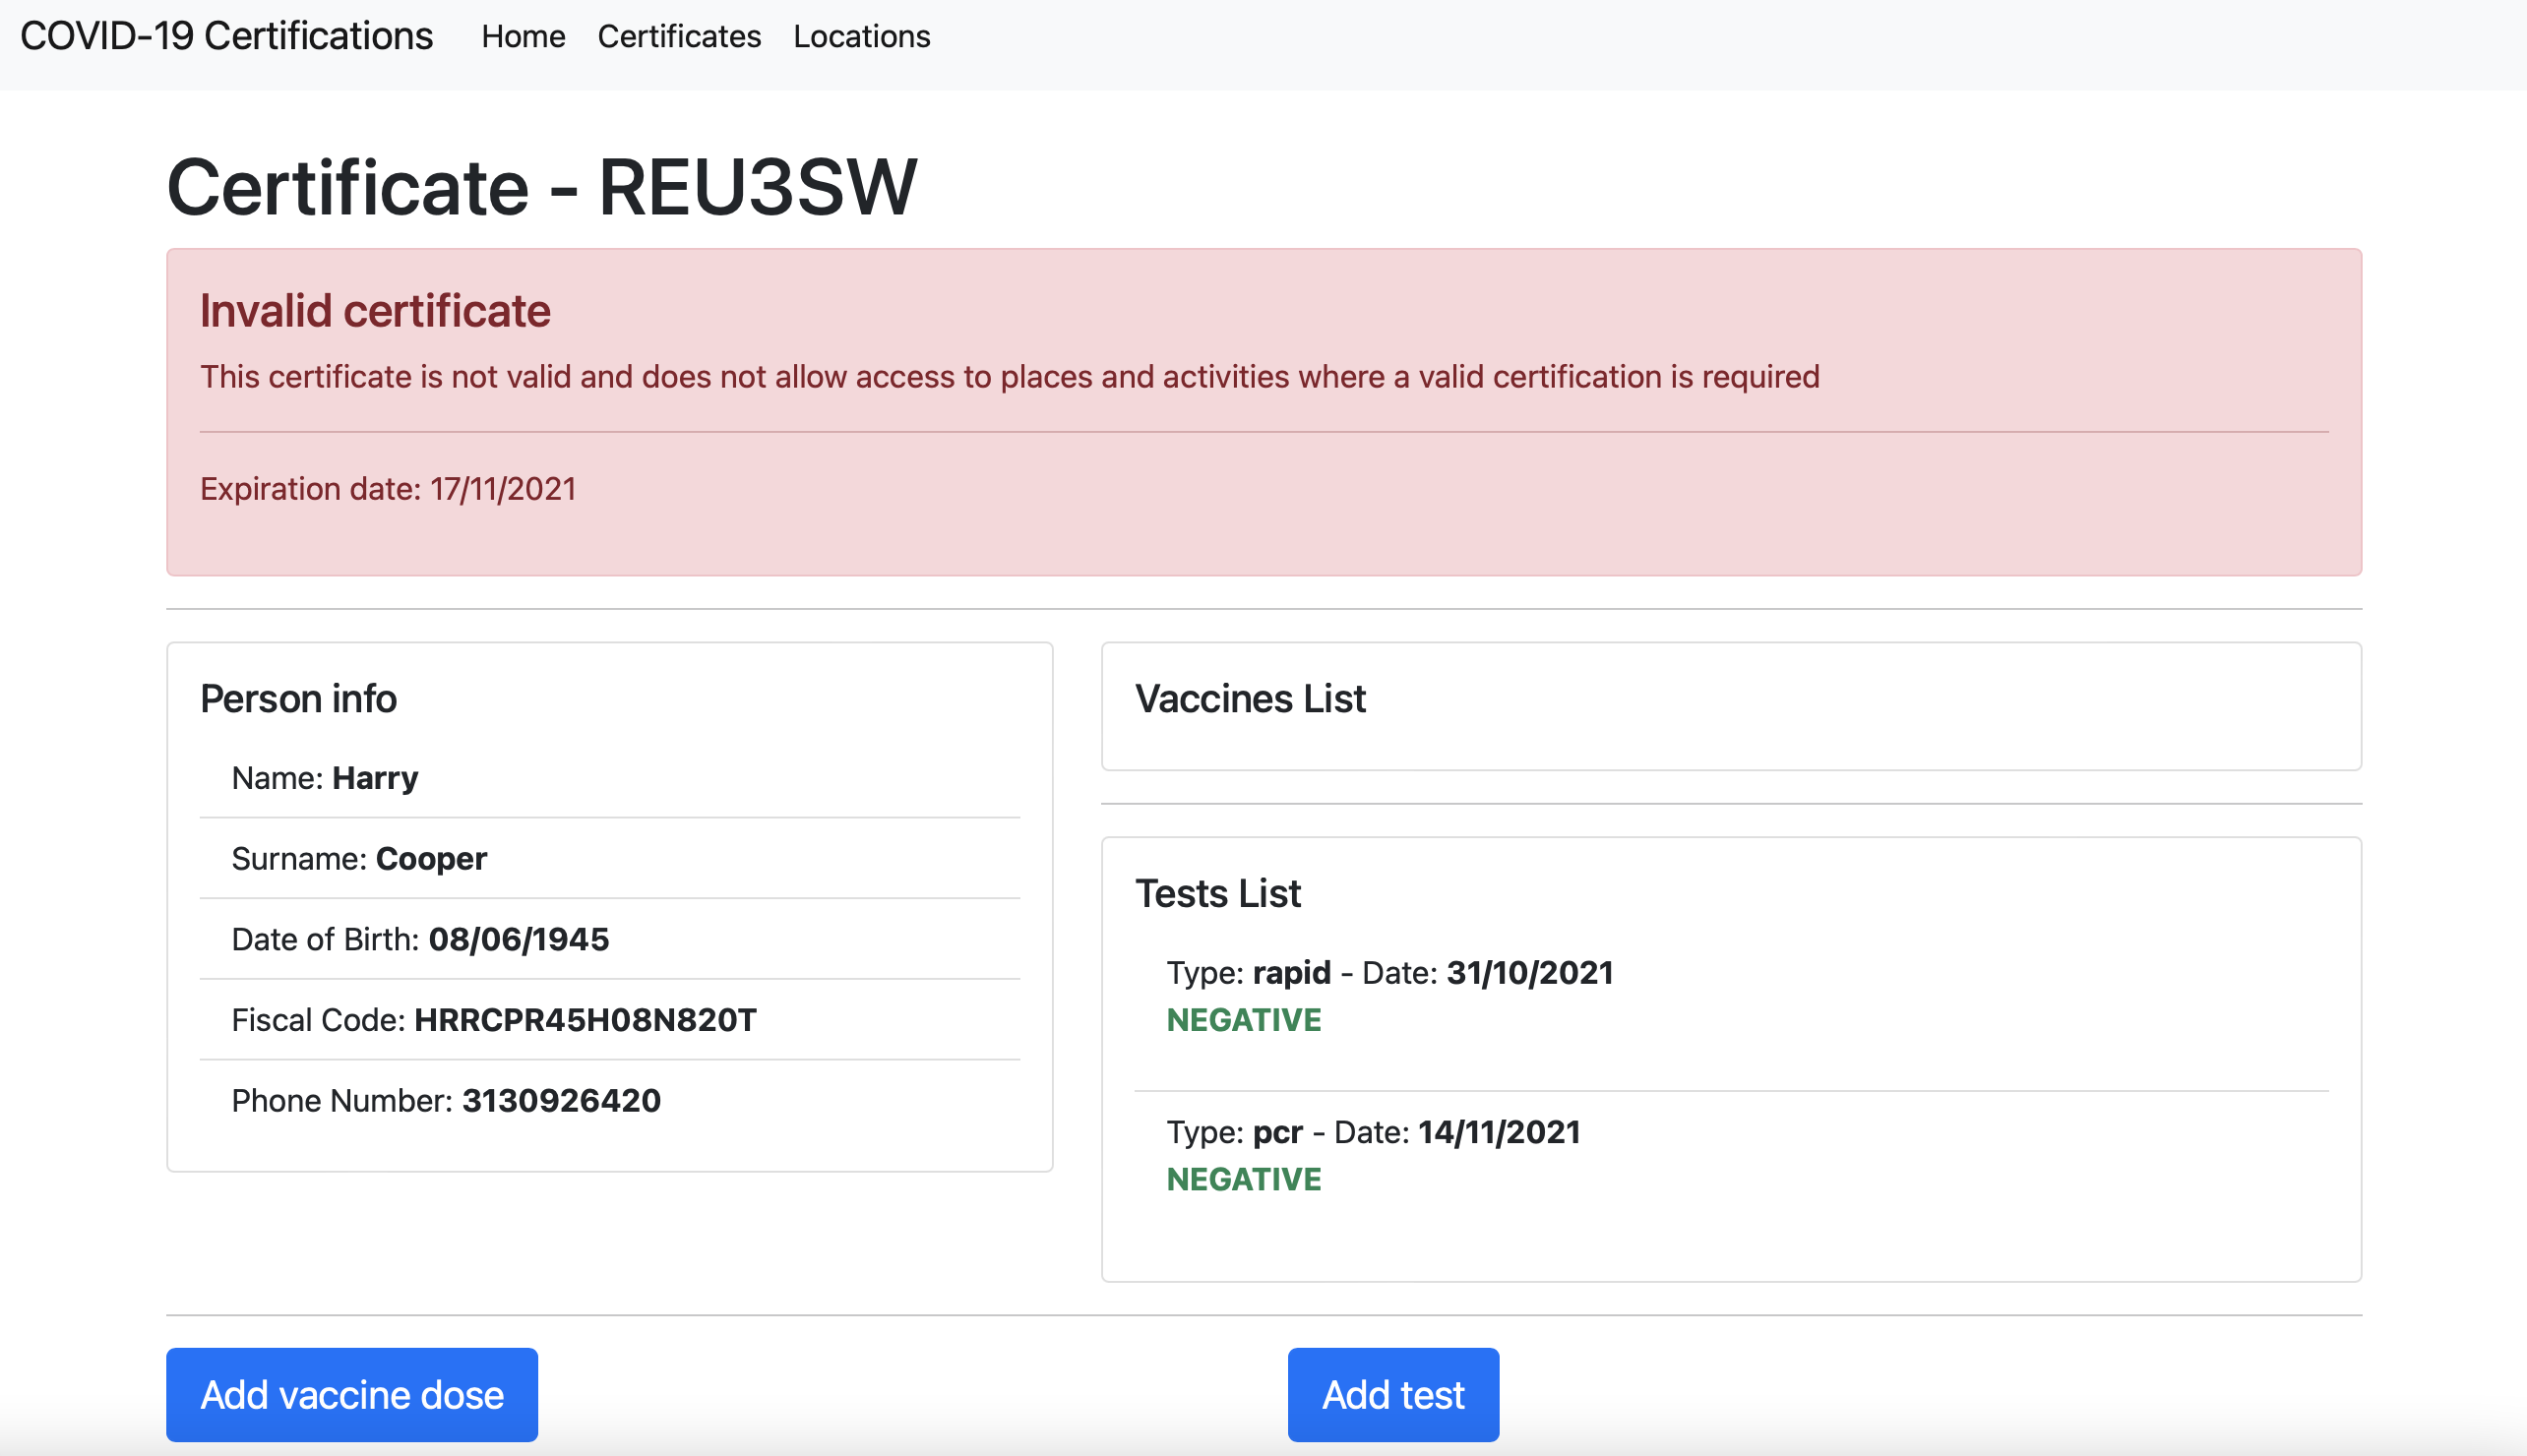
\includegraphics[scale=0.3]{screenshots/certificate.png}
    \caption{How the app shows the overview of a (invalid) certificate.}
\end{figure}
\begin{figure}[ht!]
    \centering
    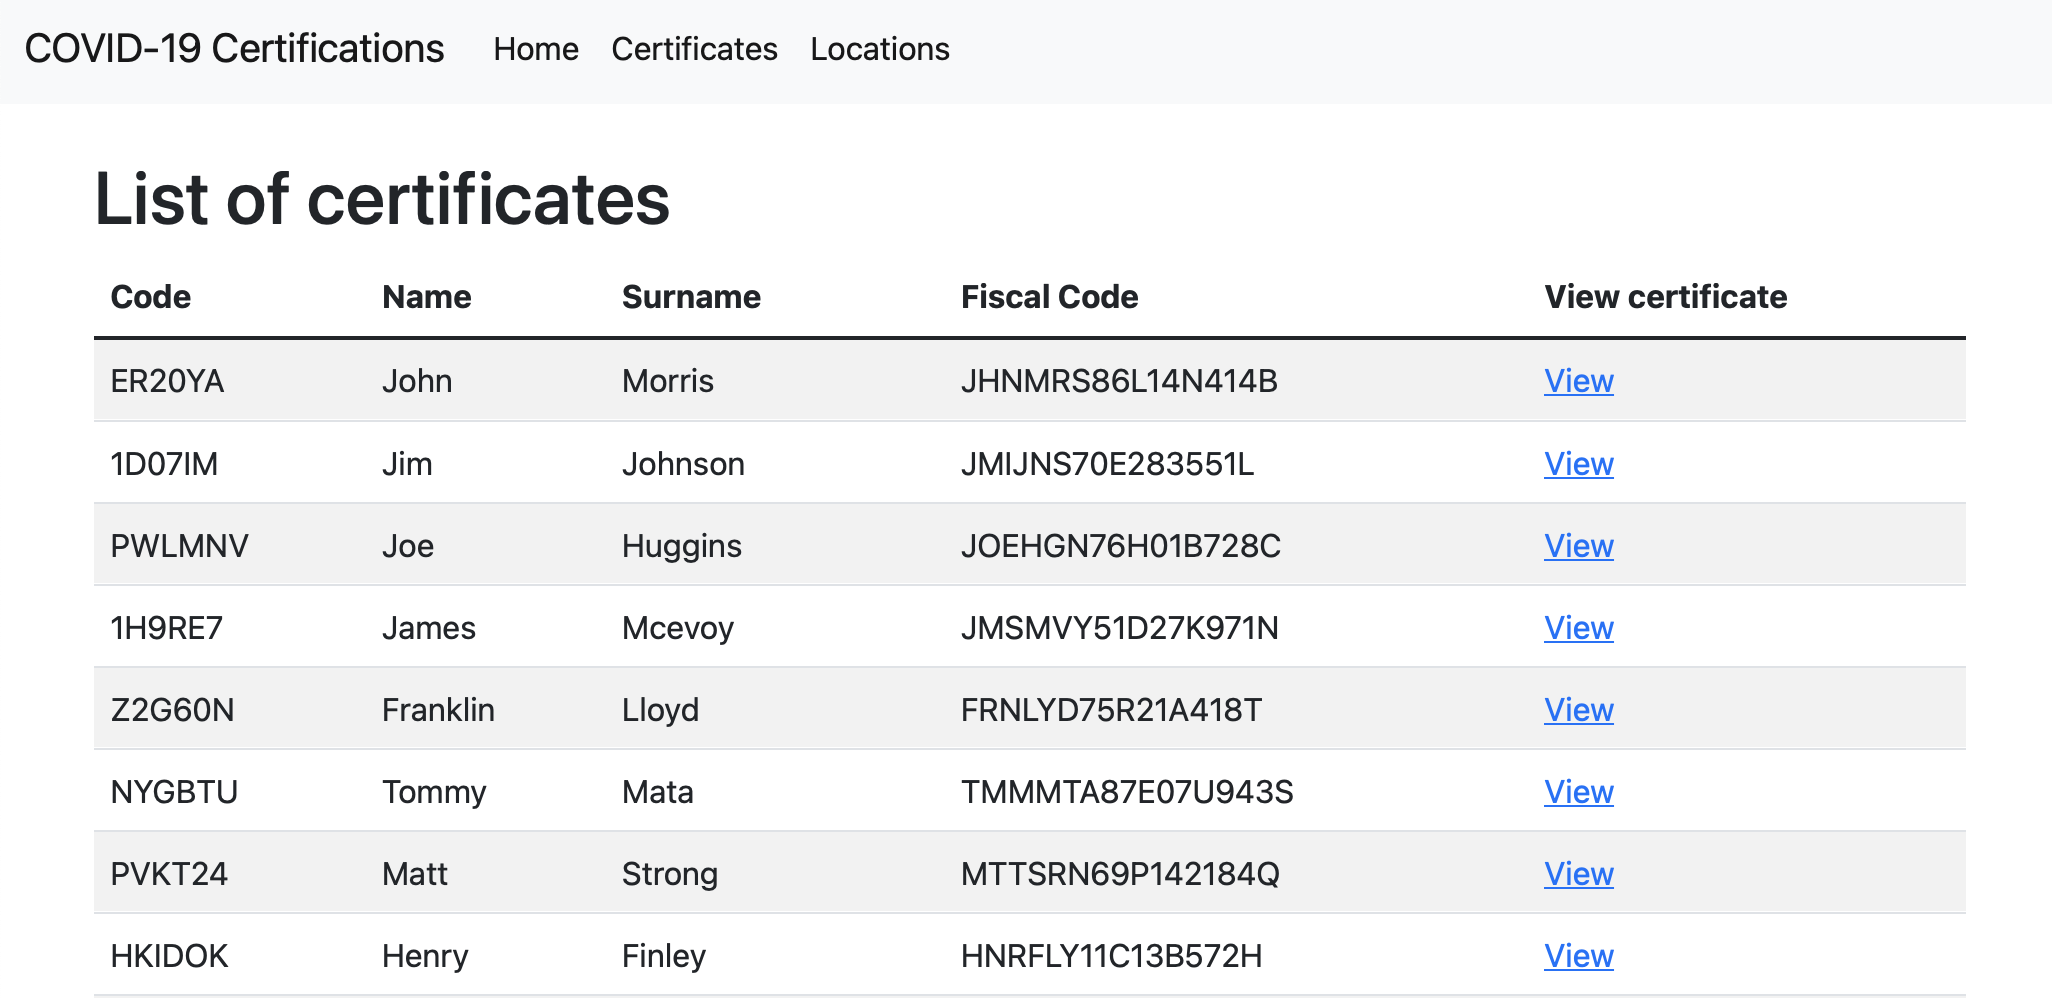
\includegraphics[scale=0.3]{screenshots/certificatelist.png}
    \caption{How the user interface shows the list of certificates.}
\end{figure}
\begin{figure}[ht!]
    \centering
    
\includegraphics[scale=0.3]{screenshots/homepage.png}
    \caption{Homepage of the application.}
\end{figure}
\begin{figure}[ht!]
    \centering
    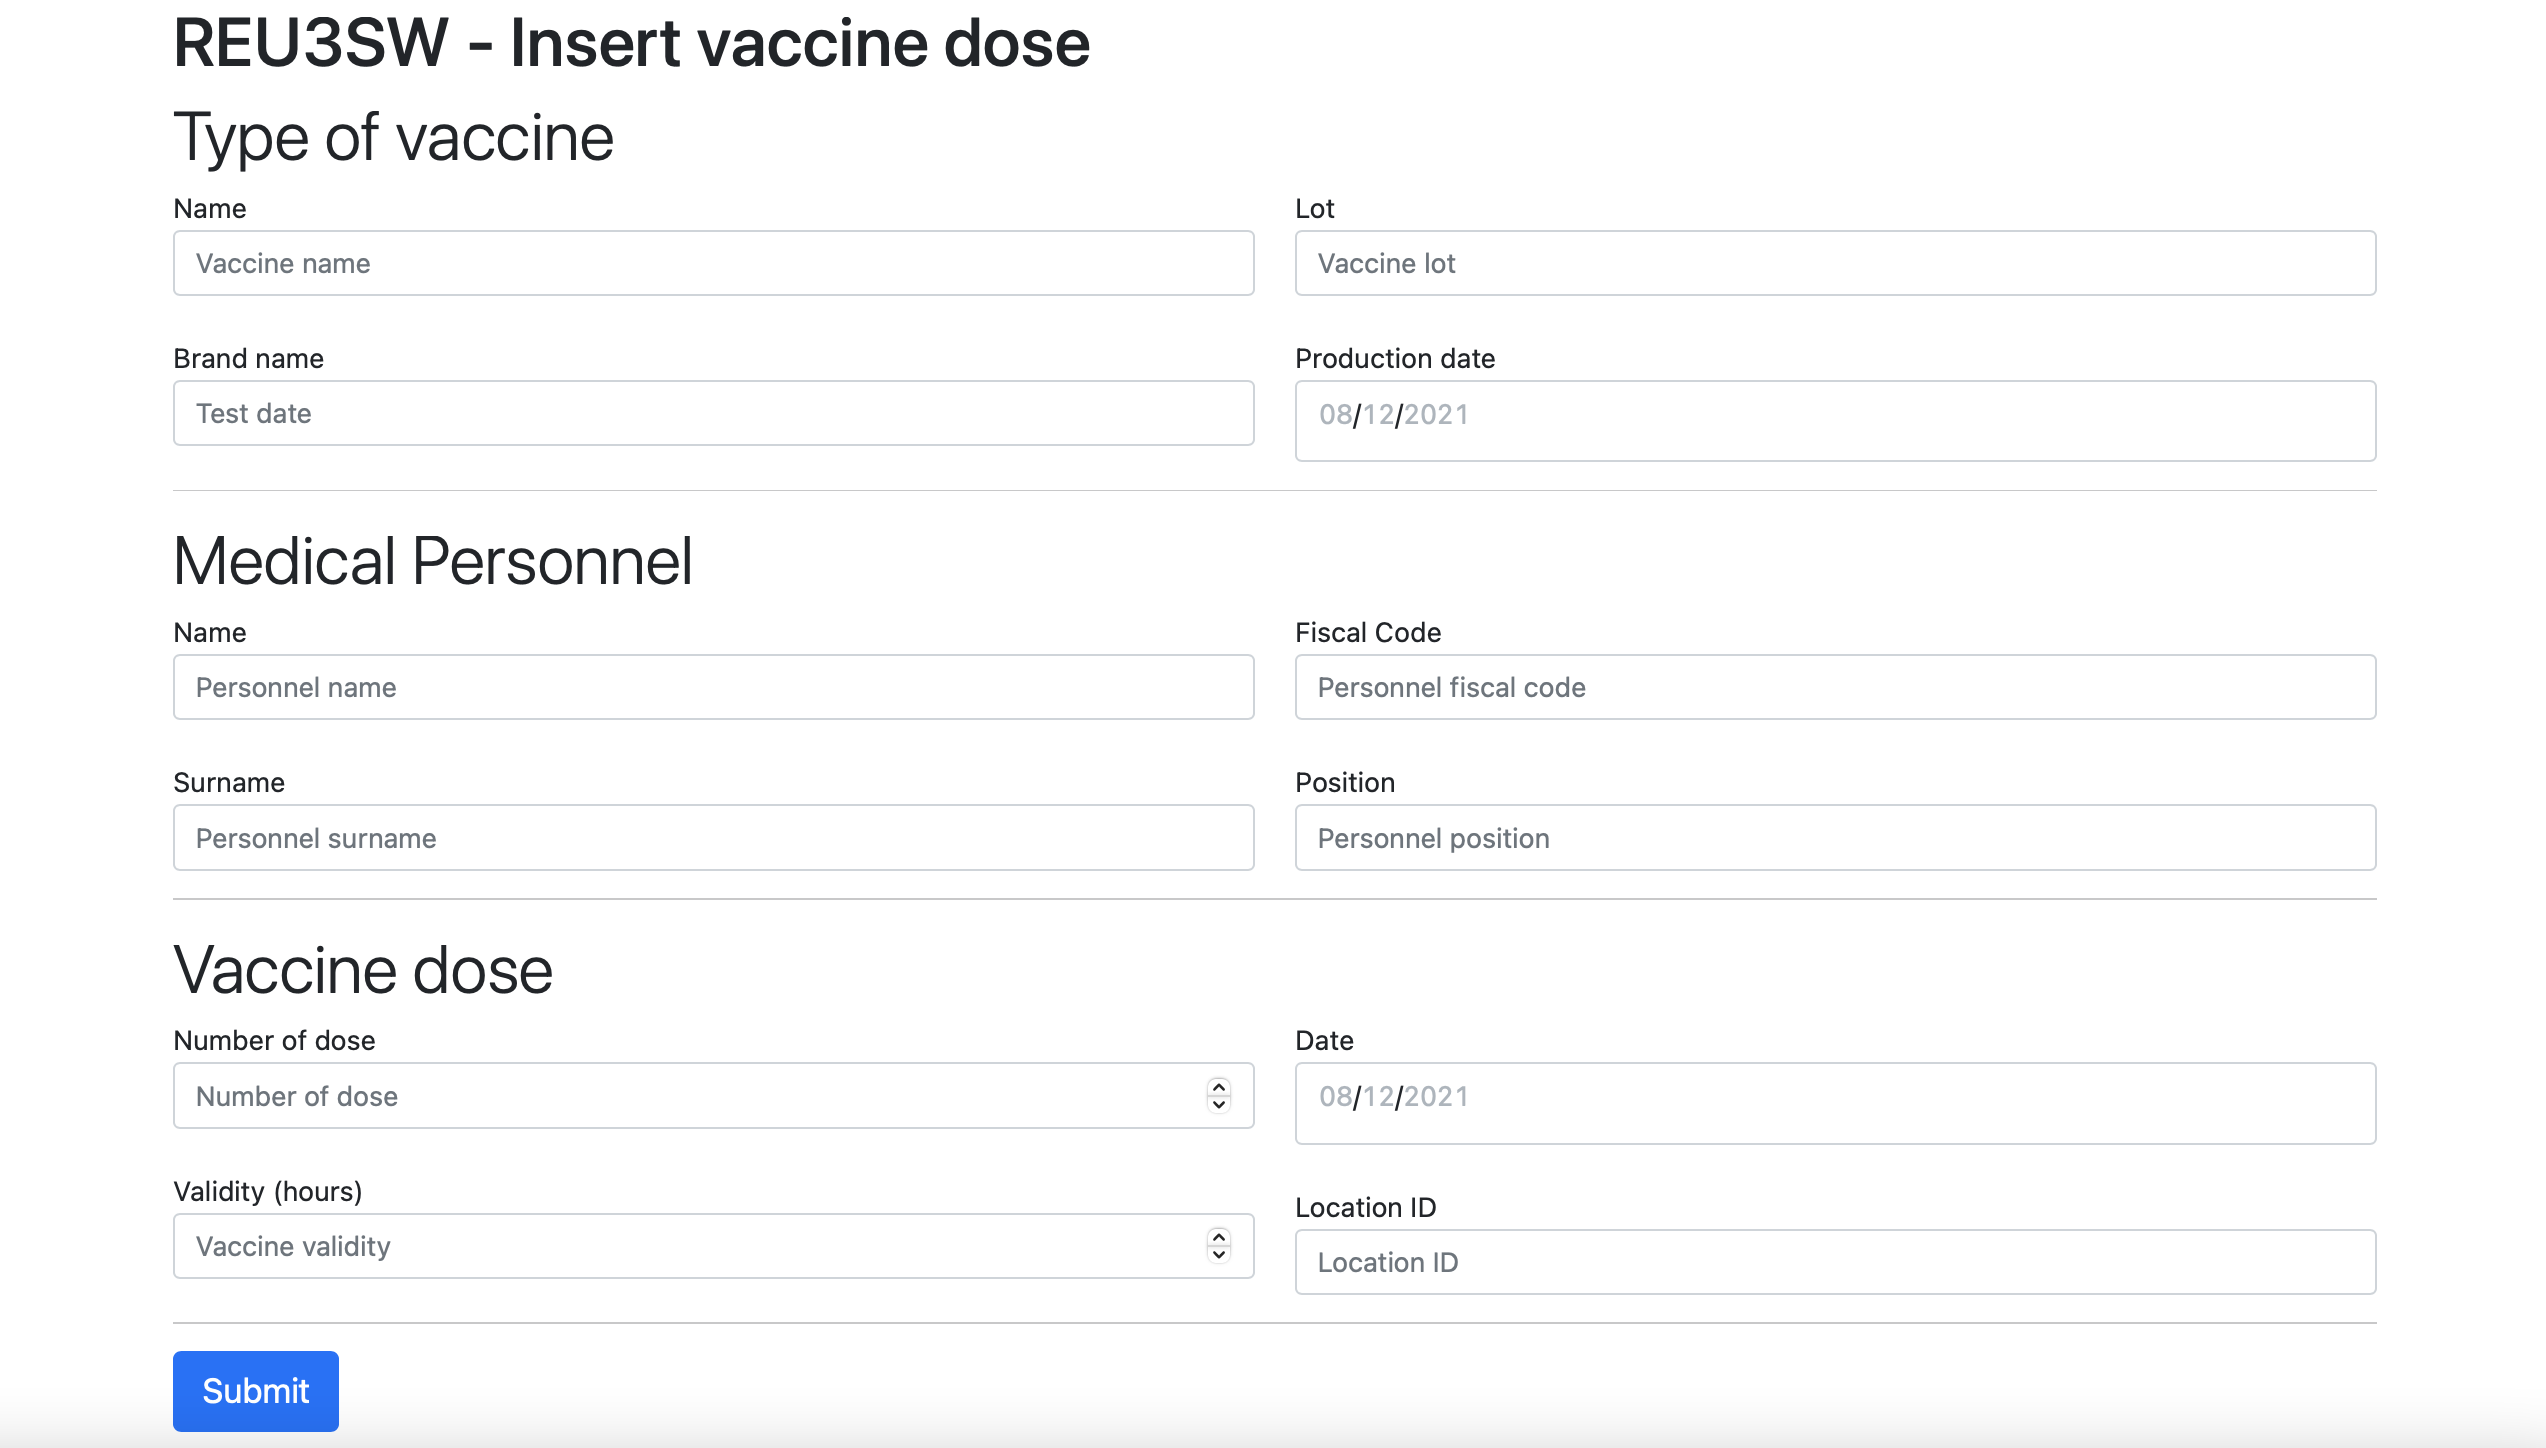
\includegraphics[scale=0.3]{screenshots/insertvaccine.png}
    \caption{Page for the insertion of a new vaccine dose to a person.}
\end{figure}
\end{document}
